\chapter{Ontology Construction and Similarity}
After getting job models by the information extraction module, the users can search jobs in the system. We notice that simple keywords matching is not a good similarity measure, because job description and r\'esum\'e are both written in human language. In these documents, even one concept can be written in different ways, and and some different concepts have close relationship. For example, Table~\ref{tab:resume_jd} shows part of the r\'esum\'e of a job seeker and part of a job description:

\begin{table}[ht]
\caption{Resume and Job Description} % title of Table
\centering % used for centering table
\begin{tabular}{ | p{8cm} | p{7cm} | }
 \hline
   \textbf{Part of Resume}                 &   \textbf{Part of Job Description}   \\ \hline

    B.S. degree in computer science \newline
    5+ years Java \newline
    2+ year   C++  \newline
    Some experience in Oracle database \newline
    Other experience like: \newline
    Hibernate, JBOSS, JUnit, Tomcat etc.
  &
  BS degree above   \newline
  4+ years Java  \newline
  Some experience of Python   \newline
    Mysql, MS-SQL   \newline
    Java web application Server   \newline
    OOA/OOD   \\
 \hline
\end{tabular}
\label{tab:resume_jd} % is used to refer this table in the text
\end{table}

If just looking at the text, we can find that the r\'esum\'e has few common words with the job description. But from the view of an experienced engineer, the candidate is pretty matching the job. Because two relational databases Oracle and Mysql are very similar; OOA/OOD is the same meaning of many years of Java and C++ experience; and Tomcat and JBOSS are both Java web applications servers. If we use key word matching, the system does not give a good matching result in this very common case.

\section{Semantic Similarity in JRSs}
In some previous studies of JRSs ontology is used as knowledge base to store knowledge and rules, which could help compare the similarity between different concepts. Liu and Dew~\cite{liu2004using} used RDF to represent and store the expertise of experts, and they used a RDF-based expertise matcher to retrieve the experts whose expertise included the required concept.

Proactive~\cite{lee2007fighting} used two kinds of ontology, job category and the company information. The system used ontology checker to classify the job information, and stored the domain knowledge and calculated the weight value in recommendations.

Fazel \cite{fazel2009semantic} used a hybrid approach to match job seekers and job postings, which takes advantage of the benefits of both logic-based and ontology-based matching. In his paper the description logics (DL) is used to represent the candidate and job opening, and the ontology is used to organize the skills in a skill taxonomy. He gave an equation to calculate the matching degree:
$$ sim\left(P ,j \right) = \sum x_{ij} \times u(ds_i) $$

where, $x_{ji}$ is the Boolean variable indicating whether desire i is satisfied by applicant $A_{j}$ in the set of all qualified applications.

Kumaran et al.~\cite{kumaran2013towards} also used ontology to calculate the similarity between job criteria and candidates's r\'esum\'e in their system~\cite{kumaran2013towards}. The similarity equation they used are:
$$ M\left ( i_1, i_2 \right ) = \frac{\sum_{k=1}^{n} Sim\left (p_{k}^{i1},  p_{k}^{i2} \right ) * W_{k}^{i2}}{\sum_{k=1}^{n} W_{k}^{i2}}  $$
The similarity function $Sim(p_1, p_2)$ is defined as follows:
$$ Sim(p1, p2) = \begin{Bmatrix}
1, & if~similarity~of~p1~and~p2 \geqslant t\\
0, & otherwise
\end{Bmatrix} $$

\section{Ontology Construction}

Before calculating the similarity between concepts, we need to construct the ontology first. Semantic web have been a hot research topic in these years, as the same time thousands of domain ontologies had been created~\cite{ding2004swoogle}. A paradigmatic example is WordNet~\cite{fellbaum1998wordnet}, which is a general purpose thesaurus, and contains more than 100,000 general English concepts. ACM has created a poly-hierarchical ontology that can be utilized in semantic web applications~\cite{acm2012class}, but it is mostly used in academic areas. DBpedia~\cite{bizer2009dbpedia} provides structured information from Wikipedia and make this information available on the Web, but its coverage is huge, and most of them is not related to job finding. Currently, there is no domain specific technology ontology built for recruiting purpose.

The domain specific technology ontology for recruiting should include a lot of technical terms, like programming language, programming library, commercial products and so on. Furthermore, there are new techniques invented everyday, so new IT terms will appear continuously. Ding et al.~\cite{ding2002ontology} gave a survey of current ontology generation approaches such as manual, semi-automatic, and automatic. Some aspects of the approaches were discussed in the paper, like the source data, concept extraction methods, ontology representation, and construction tools. Inspired by this paper, we propose a semi-automatic approach to construct the IT skill ontology, which use pattern matching approach to collect possible technical terms, and use DBpedia to verity the them.

From the observation, we found that sentences with skill requirements in job descriptions always list several skills in one the sentence, which is shown in Table ~\ref{tab:skillrequirement}. Based on this character, we propose a bootstrap approach to collect IT terms in job descriptions.  First, we manually collect about fifty terms from job descriptions, and add them to the term list. Then we use our pattern matching library to find the sentences that matching the pattern in Table \ref{tab:patterns} from a set of job descriptions. An example of a sentence which matches the pattern is shown in Table \ref{tab:termspattern}. We extract the tokens which match the star symbol from the sentences; these tokens have high probability to be technical terms. Then we could check the tokens in Dbpedia to see whether they are under the categories like software, programming language or any other technical related ones. If they are, we could classify them as terms, and add them to the terms list. After scanning all the sentences in the job description set, the term list will be larger, and we can use the larger term list to start a new iteration of scaning. This process stops when the number of found new terms is below a threshold. The process is shown Figure ~\ref{fig:gen_onto}.

\begin{table}[ht]
\caption{Some sentences Job Description} % title of Table
\centering % used for centering table
\begin{tabular}{ | p{15cm}  | }
 \hline
    1. A high-level language such as Java, Groovy, Ruby or Python; we use Java and Groovy extensively \newline
    2. HTML5/CSS3/JavaScript, web standards, jQuery or frameworks like AngularJS would be great \newline
    3. HTML CSS and Javascript a must  \newline
    4. Experience with AJAX, XML, XSL, XSLT, CSS, JavaScript, JQuery, HTML and Web Services   \\
 \hline
\end{tabular}
\label{tab:skillrequirement} % is used to refer this table in the text
\end{table}



\begin{table}[ht]
\caption{Patterns to extract terms} % title of Table
\centering % used for centering table
\begin{tabular}{   | p{8cm} |  }
 \hline
     term   , * , *,  term  \\  \hline
     term  , * , *, and  term   \\
 \hline
\end{tabular}
\label{tab:patterns} % is used to refer this table in the text
\end{table}

\begin{table}[ht]
\caption{Some sentences Job Description} % title of Table
\centering % used for centering table
\begin{tabular}{   | c | c | c | c |c | c |c | c |c | c |c | c |c | c |  }
 \hline
     Experience & with & TERM & , & *   & , & *   &, & TERM &, & and & *  \\
 \hline
     Experience & with & AJAX & , & XML & , & XSL &, & XSLT &, & and & CSS  \\
 \hline
\end{tabular}
\label{tab:termspattern} % is used to refer this table in the text
\end{table}

For example, we extract the token  ''XSL'', which currently is not in the terms list. We check the word on DBpedia by accessing the URL:http://dbpedia.org/page/XSL. If we can get the XML formatted description of XSL, and any element in ``dcterms:subject'' section has the value which is a technical category,  like ``Programming languages'', ``Markup languages'' and so on, we can indicate that the word is a technical term, and add it to the term list.

\begin{figure}[htbp]
  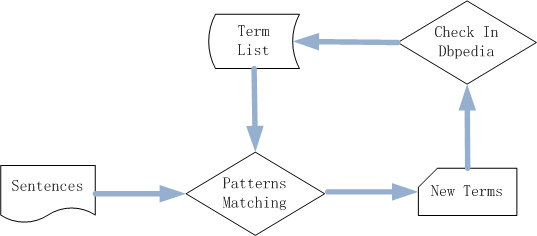
\includegraphics[scale=0.6]{images/genonto.png}
  \caption{Find Technical Terms}
  \label{fig:gen_onto}
\end{figure}

But not all the extracted terms can be verified in DBpedia, because some terms have multiple meaning in English, and the URLs of their DBpedia pages are unpredictable. For example, the word ``Python'' could be an animal name or a programming language.  The meaning of the programming language  has the DBpedia URL http://dbpedia.org/page/Python\_(programming\_language), which is hard to be predicted. In such case, we have to check the term manually.  After getting all terms, we use Protege~\cite{noy2001creating}, an open source ontology editor, to edit the domain specific ontology, and saved it in RDF format. The interface of Protege is shown in Figure~\ref{fig:Protege}. Part of the technical ontology is shown in Figure ~\ref{fig:ontology_pro}.


\begin{figure}[htbp]

  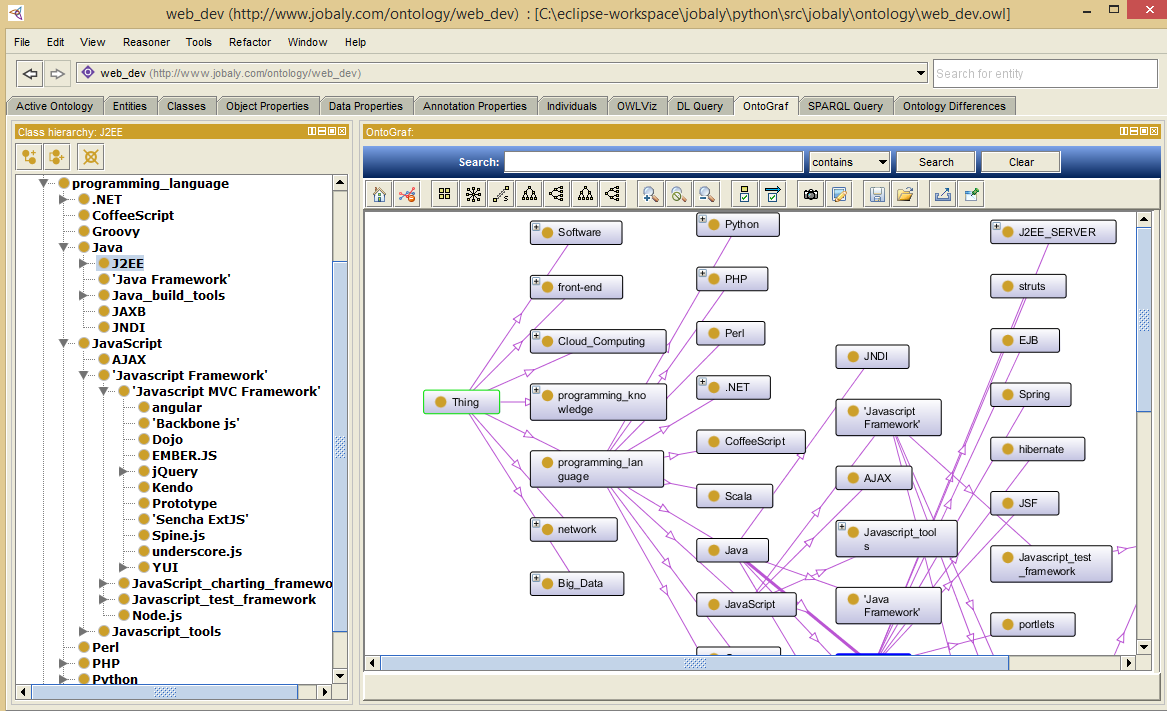
\includegraphics[scale=0.5]{images/protege.png}
  \caption{Interface of Protege}
  \label{fig:Protege}
\end{figure}

\begin{figure}[htbp]
  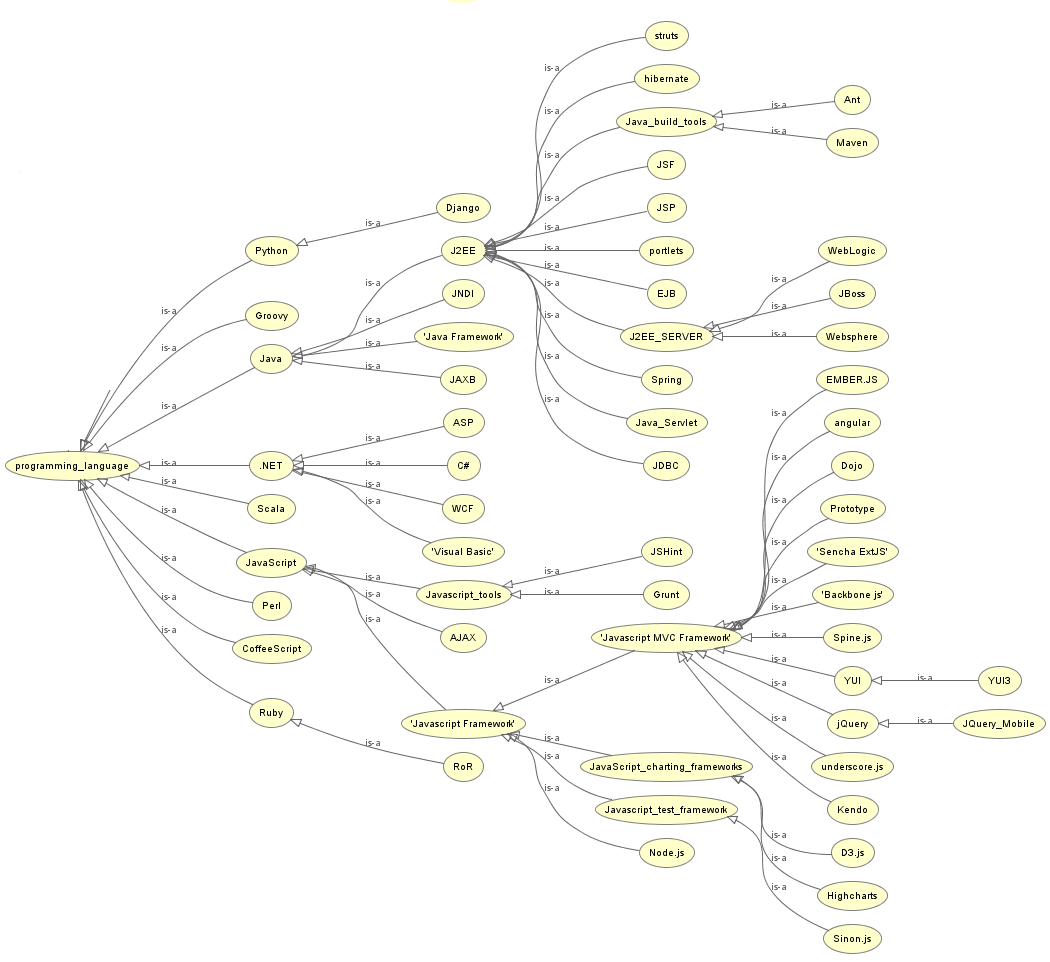
\includegraphics[scale=0.6]{images/ontology_pro.png}
  \caption{Part of Ontology}
  \label{fig:ontology_pro}
\end{figure}

\section{Ontology-based semantic similarity}

S{\'a}nchez et al. \cite{sanchez2012ontology} summarized ontology-based similarity assessment into three kinds, and gave both advantages and disadvantages of each approach. The three kinds of categories are: Edge-counting approaches, Feature-based measures, and Measures based on Information Content.


\subsection{Path-based approaches}
In path-based approaches , the ontology is viewed as a directed graph, in which the nodes are the concepts, the edges are taxonomic relation, like (is-a). Rada, et al.,~\cite{rada1989development} measure the similarity by the distance of two nodes in the graph. So the semantic distance of two concepts $a$ and $b$ will be:
$$ dis_{rad}(a,b) = min |path_i(a,b)| $$

Wu and Palmer~\cite{wu1994verbs} realized that the depth in the taxonomy will impact the similarity measure of two nodes, because the more deeper of the nodes are in the tree, the semantic distance is smaller. So they gave a new measure of ontology:
$$ sim_{w\&p}(a,b) = \frac{2 \times N_3}{N_1 + N_2 + 2 \times N_3} $$
$N_1$ and $N_2$ is the numbers of is-a links from each term to their Least Common Subsumer(LCS), $N_3$ is the number of is-a links of the LCS to the root of the ontology.

Based on the same idea, Leacock and Chodorow~\cite{leacock1998combining} also proposed a similarity measure that combined distance $Np$ between terms $a$ and $b$ and the depth $D$ of the taxonomy.
$$ sim_{l\&c}(a,b) = -\log (Np/ 2D) $$

There are some limitations of path-based approaches. First it only consider the shortest path between concept pairs, when they meet complex situation like multiple taxonomical inheritance, the accuracy of them will be low. Another problem of path-based approaches is that they assume that all links in the taxonomy have uniform distance.

\subsection{Feature-based measures}

Feature based approaches assess similarity between concepts as a function of their properties. They consider degree of overlapping between sets of ontological features, like Tversky's model~\cite{tverskyfeatures}, which subtract the non-common features from common features of two concepts.
$$  sim_{tve}(a,b) = \alpha \cdot F \left( \Psi(a) \cap   \Psi(b)  \right) - \beta  \cdot F \left( \Psi(a) \setminus   \Psi(b)  \right) - \gamma \cdot F \left( \Psi(b) \setminus   \Psi(a)  \right)  $$
Where F is salience of a set features, and $\alpha, \beta$ and $\gamma$ are weights of the contribution of each component.

Rodr{\'\i}guez and Egenhofer~\cite{rodriguez2003determining} computed similarity by sum the weighted sum of similarities between synsets, features, and neighbour concepts.
$$ sim_{re}(a,b) = w \cdot S_{synsets}(a,b) + u \cdot S_{features}(a,b) + v \cdot S_{neighborhoods}(a,b) $$

The feature-based methods consider more semantic knowledge than path-based methods. But only big ontologies/thesauri like Wordnet~\cite{miller1995wordnet} have this kind of information. Ding et al.~\cite{ding2004swoogle} had revealed that domain ontologies very occasionally model any semantic feature apart from taxonomical relationship.

\subsection{Content-based measures}
Other approaches want to overcome the limitations of edge-counting approaches are Content-based measures. Resnik~\cite{resnik1995using} proposed a similarity measure, which depends on the amount of shared information between two terms:
$$ sim_{res}(a,b) = IC(LCS(a,b))$$
LCS is the Least Common Subsumer of terms in a ontology, and IC is Information Content, which is the negative log of its probability of occurrence, $p(a)$. Lin (1998) and Jiang and Conrath (1997) extended Resnik��s work. They also considered the IC of each of the evaluated terms, and they proposed that the similarity between two terms should be measured as the ratio between the amount of information needed to state their commonality and the information needed to fully describe them.
$$ sim_{lin}(a,b)=\frac{2 \times sim_{res}(a,b)}{(IC(a)+IC(b))}$$
The are also two disadvantages of content-based measures. First these approaches cannot compute the concepts of leave nodes, because they don't have subsumers. Second if the concepts do not have enough common subsumers, their similarities are hard to be calculated.


\section{Statistical-based Ontology Similarity Measure }
In this thesis, we proposed a new statistical-based ontology similarity measure. In most job descriptions, they list many skills the positions required. From observation, we found that related skills always exist in the job description simultaneously, and the positions of them are always close, e.g. HTML and CSS are always required together, and appear in the same sentence. We could see this phenomenon in Table~\ref{tab:skillinsent}, which include some skill requirement sentences from some job descriptions.

\begin{table}[ht]
\caption{Some sentences Job Description} % title of Table
\centering % used for centering table
\begin{tabular}{ | p{15cm}  | }
 \hline
    1. A high-level language such as Java, Groovy, Ruby or Python; we use Java and Groovy extensively \newline
    2. HTML5/CSS3/JavaScript, web standards, jQuery or frameworks like AngularJS would be great \newline
    3. HTML CSS and Javascript a must  \newline
    4. Experience with AJAX, XML, XSL, XSLT, CSS, JavaScript, JQuery, HTML and Web Services   \\
 \hline
\end{tabular}
\label{tab:skillinsent} % is used to refer this table in the text
\end{table}

We can see from the Table~\ref{tab:skillinsent}, the closely related concepts are always have short distance. Based on such observation, we give a new statistical-based ontology similarity measure. If two concepts $a$ and $b$ have the same direct hypernym or one  is the hypernym of the other, the similarity between them is given:
$$ S(a,b) = \frac{  N_{a \cap b} / N_{a \cup b} }{avg(\log_2( mindis(doc,a,b) + 1 ))} $$

The numerator is the ratio of the number of documents in which the two terms exist together $(N_{a \cap b})$ to the number of documents have a least one them $(N_{a \cup b})$. The denominator is the average $\log$ value of minimum distance $mindis(doc,a,b)$ of the two terms in documents that have them both.

We set the restriction on the position of the two concepts in the ontology, because the position of the concepts in the ontology are based on their technical similarity to others. Similar techniques will be assigned into the same category, so they should share the same hypernym, and one could be a alternate to the other. For example, we put EJB and Hibernate in the same category, because they are both J2EE persistence layer technologies, and both have the O/R mapping concept. If the applicant is familiar one of them, they can master the other very quickly. Another example is Grail and Django, they are both web frameworks, and share same web design philosophies, but one of them is designed for Java web application and the other is created for Python web application. If a developer has some some experience with one of them, he/she still need spend a lot of time to learn the other to overcome the gap between programming languages. The algorithm to calculate the similarity of two concepts is in algorithm ~\ref{alg:alg_similarity}.

\begin{algorithm}
\caption{Get Stat Similarity}
\label{alg:alg_similarity}
\KwIn{$Docs$�� $term1$, $term2$}
\KwOut{$similarity$}
$total=0$;
$hastwo=0$;
$dislist=\left [ ~~ \right ]$\;
\For{$i=1;~i~\le~len(Docs);~i++$}
{
  \If{ $ Docs_i~has~at~least~one~term $ }
    {
     $ total~+=~1 $ \;
     \If{ $ Docs_i~has~both~terms $ }
        {
           $ hastwo~+=~1 $ ;
           $ mindis~=~ minimium\_distance~(Docs_i, term1, term2) $ \;
           $ dislist.~add  ~\left(  log_2( mindis + 1 ) \right) $ \;
        }
    }
}
$ factor1~=~hastwo~ /~ total $  \;
$ factor2~=~ avg(dislist) $  \;
return $factor1 ~/~ factor2$\;
$ ~~ $
\end{algorithm}

The matrix in table~\ref{tab:dismatrix1} show the similarity values among of some skills, which is gotten from 500 job descriptions. For example the skill HTML, the most relevant skills in order are CSS, Javascript, and jQuery,  which is the same from the perspective of experienced developers. The other example is Java, the most relevant skill in the matrix is JSP, which is also agree with the general technical knowledge.


\begin{table}

\caption{Skills Similarity Table 1}
\begin{tabular}{ c | c c c c c c   }
 \hline
  Term       &  Java  &  JDBC  & Spring & Hibernate & MySql  & Oracle   \\  \hline
  Java   &   1    & 0.0523 & 0.091  &   0.0458  & 0.0339 & 0.0608    \\  \hline
    JDBC   & 0.0523 &   1    & 0.0525 &   0.0799  & 0.006  & 0.0616   \\  \hline
   Spring  & 0.091  & 0.0525 &   1    &   0.2008  & 0.0194 & 0.0878   \\  \hline
 Hibernate & 0.0458 & 0.0799 & 0.2008 &     1     & 0.0073 & 0.115    \\  \hline
   MySql   & 0.0339 & 0.006  & 0.0194 &   0.0073  &   1    & 0.049    \\  \hline
   Oracle  & 0.0608 & 0.0616 & 0.0878 &   0.115   & 0.049  &   1      \\  \hline
 \hline
\end{tabular}
\label{tab:dismatrix1}
\end{table}


\begin{table}

\caption{Skills Similarity Table 2 }
\begin{tabular}{ c | c c c c c c c c }
 \hline
  Term       & Javascript & jQuery &  HTML  &  CSS   &  Java  & Python &  Ruby  &  JSP    \\  \hline
  Javascript &     1      & 0.1981 & 0.2087 & 0.2439 & 0.0665 & 0.0189 & 0.023  & 0.0253   \\
    jQuery   &   0.1981   &   1    & 0.0979 & 0.1328 & 0.0439 & 0.0142 & 0.0266 & 0.0232    \\
     HTML    &   0.2087   & 0.0979 &   1    & 0.3569 & 0.0473 & 0.0175 & 0.023  & 0.0103   \\
     CSS     &   0.2439   & 0.1328 & 0.3569 &   1    & 0.0537 & 0.0153 & 0.0181 & 0.015    \\
     Java    &   0.0665   & 0.0439 & 0.0473 & 0.0537 &   1    & 0.0498 & 0.0287 & 0.075    \\
    Python   &   0.0189   & 0.0142 & 0.0175 & 0.0153 & 0.0498 &   1    & 0.1333 & 0.0025   \\
     Ruby    &   0.023    & 0.0266 & 0.023  & 0.0181 & 0.0287 & 0.1333 &   1    & 0.012    \\
     JSP     &   0.0253   & 0.0232 & 0.0103 & 0.015  & 0.075  & 0.0025 & 0.012  &   1      \\
 \hline
\end{tabular}
\label{tab:dismatrix2}
\end{table}

\section{Combine Keyword Search and Ontology Matching }

Using ontology matching, the system can give job seekers some jobs appropriate to their background. But, in some cases, job seekers have their own preference when choosing jobs. These cases are not very rare, for example, some people may want to try new positions or industries that they have little or no experience, because they are bored with current positions, or they want to learn some perspective technologies. Considering such situations, we add a new search feature to the system, which combine the traditional keyword searching and our ontology matching approach. First, the user need to upload their r\'esum\'e, and then they can use keywords to search jobs. The system will get the jobs that contain the keywords, and the jobs are ranked by their similarity values to the user's r\'esum\'e. The keywords represent user's preference, that jobs satisfied this criteria will be returned, and the ontology similarity become the ranking algorithm, which make the top items of the searching result more relevant to user.
